\documentclass[a4paper, 12pt]{article}
\usepackage{./common/style}

\begin{document}
	\docNumber{RU.17701729.05.06-01 34 01} \docFormat{Руководство оператора} \student{программы \enquote{Программная инженерия}}{Д.А. Щербаков} \project{Программа для визуализации данных о климате и погоде помощью JavaScript.}
	\supervisor{Доцент департамента программной инженерии}{Р.А. Родригес Залепинос} \firstPage
	\newpage
	\thirdPage

	\newpage

	\section{Объект испытаний}
	\subsection{Наименование программы}
	Полное наименование -- \enquote{Программа для визуализации данных о климате и погоде помощью JavaScript}. Наименование
	на английском языке -- \enquote{Program for Visualizing Climate and Weather Data on JavaScript}. Условное обозначение
	-- \enquote{Climap}.

	\subsection{Краткая характеристика области применения программы}
	Программа для визуализации данных климата и погоды предназначена для использования в сфере метеорологии, географии и экологии.
	Она обеспечивает возможность анализа и представления динамики климатических параметров и погодных условий в удобном
	графическом виде. Область применения программы охватывает научно-исследовательские учреждения, государственные
	метеорологические службы, а также образовательные организации и частные компании, занимающиеся исследованиями в
	области климата и погоды.

	\section{Цель испытаний}
	Целью испытаний является:
	\begin{itemize}
		\item Проверка программного проекта \enquote{Программа для визуализации данных о климате и погоде помощью JavaScript}
			на соответствие требованиям, указанным в техническом задании.

		\item Проверка эксплуатационной и регламентной документации программного проекта \enquote{Программа для визуализации данных о климате и погоде помощью JavaScript}.

		\item Принятие решения о качестве разработанного программного обеспечения и возможности введения его в эксплуатацию.
	\end{itemize}

	\section{Требования к программе}

	\subsection{Требования к функциональным характеристикам}
	Программа должна обеспечивать выполнение следующих функций:
	\begin{enumerate}
		\item Предоставлять пользователю доступ к наборам климатических и погодных данных из различных источников,
			автоматически обновлять список доступных данных.

		\item Позволять пользователю настроить визуализацию данных на карте, в виде графика или текстовых характеристик в
			зависимости от размерности и типа данных в конкретном источнике. Пользователь может выбрать тип отображения,
			цветовую палитру, а также необходимые для отображения дату и время.

		\item Отрисовывать данные в соответствующем входным параметрам виде с сохранением отзывчивости интерфейса.

		\item Использовать механизмы локального кэширования данных для сокращения количества обращений к источникам данных.

		\item Сохранять входные параметры и восстанавливать их при перезагрузке программы (страницы в интернет-обозревателе).
	\end{enumerate}

	\subsection{Требования к надежности}
	\label{subsection:3_2} При любом вводе программа не должна завершаться аварийно, за исключением случаев, когда ресурсы
	устройства не соответствуют минимальным требованиям и не позволяют обработать большой массив данных -- в таком случае
	веб-обозреватель может внезапно прервать работу программы. Ошибки программы не должны приводить к экстренному завершению
	работы программы или недоступности функций. Ошибки, вызванные внешними условиями, которые возможно обработать, такими как
	обрыв интернет соединения во время загрузки данных, должны быть обработаны и сообщены пользователю. Ошибки, возникшие
	в следствие ошибок среды выполнения, которые не могут быть обработаны программой (например, ошибка веб-обозревателя или
	операционной системы) могут произвольным образом влиять на выполнение программы, но программа должна возобновить работу
	в корректном состоянии после устранения ошибки среды и перезагрузки. Допускаются краткосрочные замедления в работе
	программы во время обработки массивов данных, но в остальных состояниях пользовательский интерфейс должен оставаться отзывчивым.

	\section{Требования к программной документации}
	Состав программной документации включает в себя:
	\begin{enumerate}
		\item \enquote{Программа для визуализации данных о климате и погоде помощью JavaScript}. Техническое задание.

		\item \enquote{Программа для визуализации данных о климате и погоде помощью JavaScript}. Руководство оператора.

		\item \enquote{Программа для визуализации данных о климате и погоде помощью JavaScript}. Программа и методика испытаний.

		\item \enquote{Программа для визуализации данных о климате и погоде помощью JavaScript}. Текст программы.
	\end{enumerate}

	Все перечисленные документы должны соответствовать требованиям ГОСТ-19 <<Единая система программной документации>> \cite{ESPD}.

	\section{Состав и порядок испытаний}
	\subsection{Технические средства}
	Испытания производятся на персональном компьютере, подключенном к сети <<Интернет>> с широким пропускным каналом (не менее
	100 МБит/с). Устройство соответствует следующим требованиям:
	\begin{enumerate}
		\item Восьми- или более ядерный процессор с максимальной тактовой частотой от 3.2 ГГц.

		\item 16 Гб ОЗУ типа DDR4 или лучше.

		\item Твердотельный накопитель с объемом от 256 Гб.

		\item Устройство ввода для управления указателем.

		\item Монитор с разрешением не менее $1920\times 1080$ точек.
	\end{enumerate}

	\subsection{Информационные средства}
	Испытания проводятся на современных операционных системах, таких как Windows 10 и macOS 14.x \enquote{Sonoma}. Программа
	запускается в браузере \enquote{Google Chrome} версии 124 или совместимом аналоге.

	\subsection{Порядок испытаний}

	Испытания объединены в непересекающиеся блоки испытаний. Перед каждым блоком необходимо перезагрузить программу, предварительно
	очистив сохраненные данные программы. Каждый блок может тестироваться отдельно и независимо, но внутри блока все испытания
	должны проводиться последовательно. Конкретные шаги испытаний описаны в разделе \ref{section:6}. Ниже приведена таблица
	с блоками и испытаниями.

	\begin{table}[h]
		\setlength{\extrarowheight}{7pt}
		\begin{tabularx}
			{\textwidth}{|X|X|X|} \hline \textbf{Блок} & \textbf{Испытания} & \textbf{Примечания} \\ \hline \multirow{5}{\hsize}{Основной функционал с настройками по-умолчанию}
			& Запуск программы & \multirow{5}{\hsize}{Данные испытания предназначены для тестирования базового функционала программы с настройками по-умолчанию}
			\\ \cline{2-2} & Работа с картой & \\ \cline{2-2} & Выбор даты & \\ \cline{2-2} & Выбор отображения карты & \\
			\cline{2-2} & Перезапуск программы & \\ \hline

			\multirow{7}{\hsize}{Основной функционал программы с пользовательскими слоями} & Запуск программы & \multirow{8}{\hsize}{Расширенный набор испытаний, включающий испытания разнообразных настроек, а также поведение в экстремальных ситуациях}
			\\ \cline{2-2} & Удаление слоев & \\ \cline{2-2} & Добавление одного слоя & \\ \cline{2-2} & Добавление второго слоя & \\ \cline{2-2} & Комбинации настроек слоев & \\ \cline{2-2} & Симуляция неисправностей & \\ \cline{2-2} &
			Симуляця замедления быстродействия & \\ \cline{2-2} & Перезапуск программы & \\ \hline

			% \multirow{4}{\hsize}{Работа с пользовательскими данными} & Запуск программы & \multirow{4}{\hsize}{Тестирование функционала на заранее неизвестных наборах данных}
			% \\ \cline{2-2} & Добавление слоя из файла & \\ \cline{2-2} & Неисправный файл & \\ \cline{2-2} & Перезапуск программы
			% & \\ \hline
		\end{tabularx}
		\caption{Блоки и порядок испытаний}
	\end{table}
	\section{Методы испытаний}
	\label{section:6}

	Все испытания проводятся методом ручного тестирования функционала программы. Тестировщик выполняет инструкции,
	указанные в описанных испытаниях.

	\subsection{Основной функционал с настройками по-умолчанию}
	\subsubsection{Запуск программы}
	\label{subsubsection:6:1:1} Открыть браузер, ввести в адресную строку \href{https://climap.pages.dev}{climap.pages.dev},
	перейти по введенному адресу. \\ \textbf{Ожидаемое поведение:} загрузка сайта и отображение основного интерфейса с
	настройками по-умолчанию.

	\subsubsection{Работа с картой}
	Проверить функционал манипуляции картой с помощью указателя, а именно:
	\begin{itemize}
		\item Перемещение камеры с помощью захвата карты с нажатой левой кнопкой мыши и движением в разные стороны. \\
			\textbf{Ожидаемое поведение:} картой можно управлять с помощью указателя и кнопок мыши.

		\item Изменение масштаба карты с помощью колеса прокрутки. \\ \textbf{Ожидаемое поведение:} масштаб изменяется предсказуемым
			образом с помощью колеса прокрутки, существуют предельные значения масштаба.
	\end{itemize}

	\subsubsection{Выбор даты}
	\begin{itemize}
		\item Обновление карты соответственно выбранной дате и времени: наблюдать за индикатором загрузки возле названий
			источников данных, а также отображаемыми данными на карте при выборе даты и времени. \\ \textbf{Ожидаемое
			поведение:} при выборе даты и времени набор данных обновляется - сначала начинается загрузка, а после меняются
			значения, отображенные на карте.

		\item Выбор даты с помощью поля ввода даты:
			\begin{itemize}
				\item Выбор с помощью виджета календаря по нажатии на поле ввода даты. \\ \textbf{Ожидаемое поведение:} календарь
					открывается, можно выбрать дату, даты соответствуют действительным, есть предельные значения, соответствующие параметрам
					наборов данных.

				\item Выбор даты вводом текста в поле выбора даты. \\ \textbf{Ожидаемое поведение:} в поле ввода даты можнно ввести
					только корректные значения (соответствующие календарю).
			\end{itemize}

		\item Выбор времени из выпадающего списка: попробовать ввести различные значения в поле времени с помощью клавиатуры
			или выбрать из выпадающего списка. \\ \textbf{Ожидаемое поведение:} можно выбрать время от 0 до 23 часов ровно из
			выпадающего списка, также соответствующее время можно ввести вручную. При вводе времени, отличающегося от возможного,
			время округляется до ближайшего допустимого значения.
	\end{itemize}

	\subsubsection{Перезапуск программы}\label{subsubsection:6:1:4}
	\begin{itemize}
		\item Перезагрузить страницу в браузере без очистки данных. \\ \textbf{Ожидаемое поведение:} выбранные настройки даты,
			наборов данных и отображения сохраняются.

		\item Очистить данные и перезагрузить страницу: открыть инструменты разработчика, на вкладке \enquote{Application}
			$\rightarrow$ \enquote{Local storage} $\rightarrow$ \enquote{https://climap.pages.dev} нажать \enquote{$\times$},
			затем перезагрузить страницу. \\
			\textbf{Ожидаемое поведение:} настройки вернулись к изначальным.
	\end{itemize}

	\subsection{Основной функционал программы с пользовательскими слоями}
	\subsubsection{Запуск программы}
	Повторить пункт \ref{subsubsection:6:1:1}.

	\subsubsection{Удаление слоев}
	Для каджого добавленного слоя повторить:
	\begin{itemize}
		\item Нажать \enquote{\vdots} справа от названия слоя.
		\item Нажать на красную кнопку \enquote{Удалить слой} (\enquote{Remove layer}) в верхней части всплывающего окна.
	\end{itemize}
	\textbf{Ожидаемое поведение:} слой пропадает из списка, а его визуальное отображение пропадает с карты.

	\subsubsection{Добавление одного слоя}
	\begin{itemize}
		\item Нажать \enquote{Добавить слой} (\enquote{Add later}).
		\item Выбрать значение: \enquote{ERA5-Land hourly / 2m temperature} в поле \enquote{Данные} (\enquote{Product}).
		\item Нажать \enquote{Сохранить} (\enquote{Save}).
	\end{itemize}
	\textbf{Ожидаемое поведение:} добавлен новый слой с индикатором загруки. После загрузки слой отобразится на карте.

	\subsubsection{Добавление второго слоя}
	\begin{itemize}
		\item Нажать \enquote{Добавить слой} (\enquote{Add later}).
		\item Выбрать значение: \enquote{ERA5-Land hourly / 2m temperature} в поле \enquote{Данные} (\enquote{Product}).
		\item Выбрать значение: \enquote{Контур} (\enquote{Contour}) в поле \enquote{Тип} (\enquote{Type}).
		\item Нажать \enquote{Сохранить} (\enquote{Save}).
	\end{itemize}
	\textbf{Ожидаемое поведение:} добавлен новый слой с индикатором загруки. После загрузки слой отобразится на карте. Одновременно на карте будут отображаться два слоя.

	\subsubsection{Комбинация настроек слоев}
	\begin{itemize}
		\item Нажать \enquote{\vdots} справа от названия первого сверху слоя.
		\item Изменить значение \enquote{Непрозрачность} (\enquote{Opacity}) до 1,0.
		\item Выбрать палитру \enquote{Viridis} в поле \enquote{Цвета} (\enquote{Цвета}).
		\item Ввести \enquote{Температура} в поле \enquote{Название слоя} (\enquote{Layer name}).
		\item Нажать \enquote{Сохранить} (\enquote{Save}).
	\end{itemize}
	\textbf{Ожидаемое поведение:} изменится название слоя в списке. Изменится отображение слоя с заливкой на карте в соответствии с новыми настройками.

	Повторить действия со наибольшим числом доступных комбинаций. Повторить со вторым слоем.

	\subsubsection{Симуляция неисправностей}
	\begin{itemize}
		\item Открыть инструменты разработчика, на вкладке \enquote{Network} выбрать замедление сети: \enquote{Offline}.
		\item Изменить дату или время в настройках приложения на ту, которая еще не использовалась.
	\end{itemize}
	\textbf{Ожидаемое поведение:} загрузка обновленных данных не удалась, рядом с текущими слоями присутствует индикатор ошибки.

	\subsubsection{Симуляция замедления быстродействия}
	\begin{itemize}
		\item Открыть инструменты разработчика, на вкладке \enquote{Performance} выбрать замедление быстродействия процессора: \enquote{4x slowdown}.
		\item Открыть инструменты разработчика, на вкладке \enquote{Performance} выбрать замедление быстродействия сети: \enquote{Fast 3G}.
		\item Изменить дату или время в настройках приложения на ту, которая еще не использовалась.
	\end{itemize}
	\textbf{Ожидаемое поведение:} загрузка обновленных данных проходит успешно, но заметно медленнее, чем раньше.

	\subsubsection{Перезапуск программы}
	Повторить пункт \ref{subsubsection:6:1:4}.

	\newpage

	\section{Список источников}
	\begingroup
	\renewcommand{\section}[2]{}
	\bibliographystyle{ugost2008}
	\bibliography{./common/references}
	\endgroup


	\addition{Отчет об испытаниях}
	\subsection{Основной функционал с настройками по-умолчанию}
	Все испытания успешно пройдены.

	\begin{itemize}
		\item Запуск программы \\ Программа запустилась, слои по-умолчанию отображаются
		\item Работа с картой \\ Весь функционал карты доступен
		\item Выбор даты \\ Все возможности выбора даты работают правильно, доступные даты определяются автоматически, данные обновляются при выборе даты
		\item Перезапуск программы \\ Настройки даты и отображения карты сохраняются при перезапуске
	\end{itemize}

	\begin{figure}[htbp]
		\centering
		\subfloat{
        	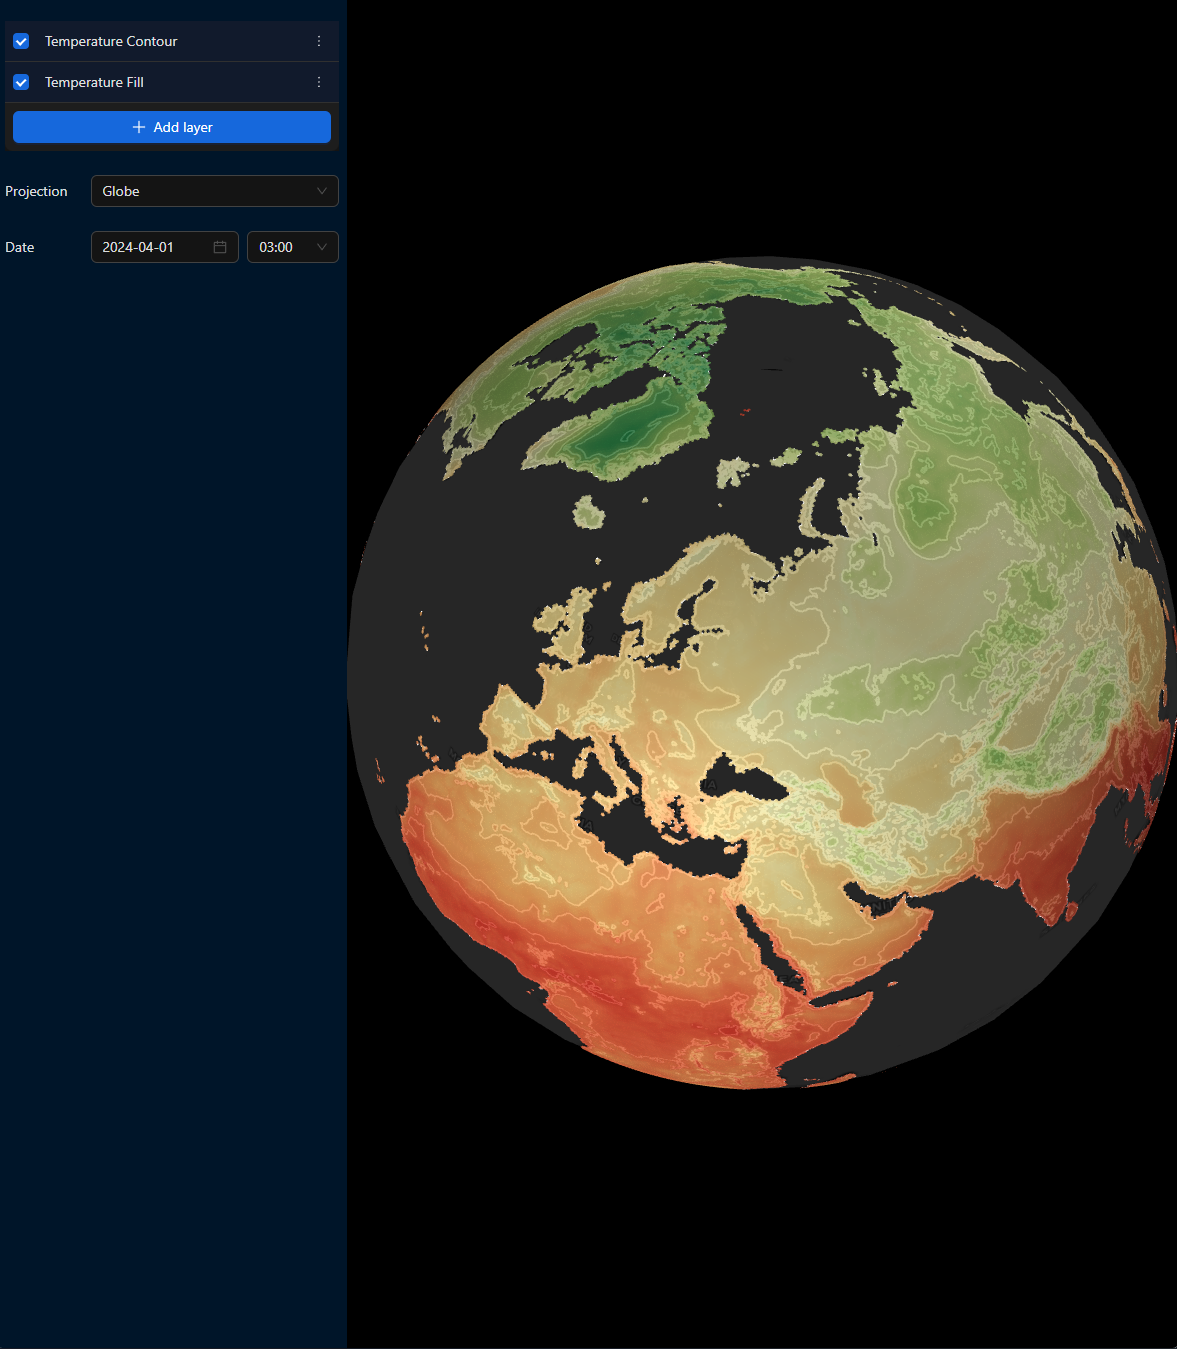
\includegraphics[width=0.3\textwidth]{assets/test1.png}
        	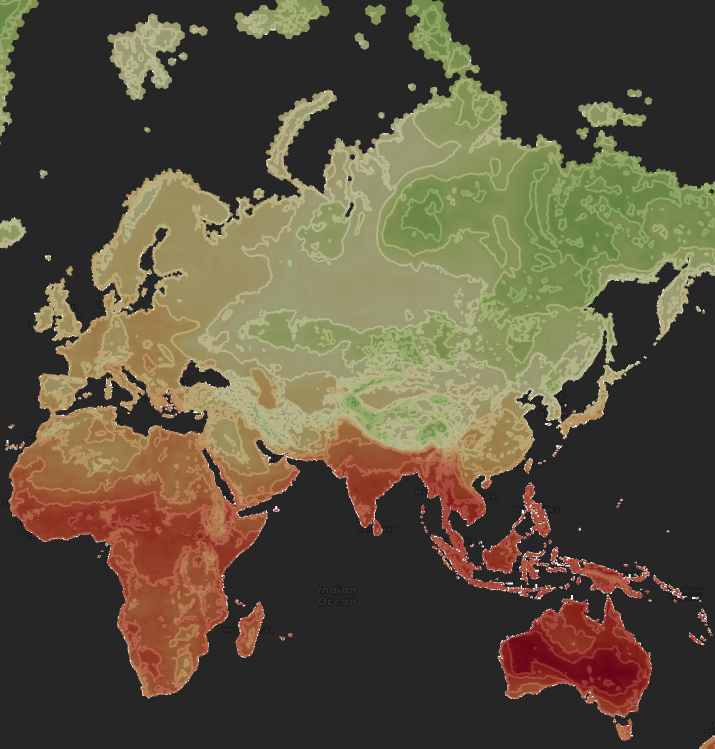
\includegraphics[width=0.3\textwidth]{assets/test2.png}
        	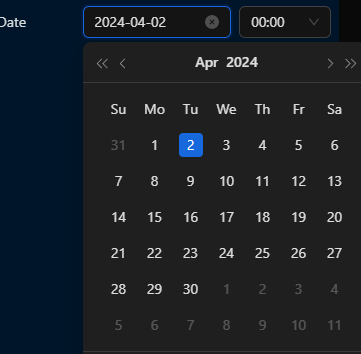
\includegraphics[width=0.3\textwidth]{assets/test3.png}
		}
		\caption{Снимки экрана}
	\end{figure}
	\subsection{Основной функционал программы с пользовательскими слоями}
	Все испытания успешно пройдены.

	\begin{itemize}
		\item Запуск программы \\ Программа запустилась, слои по-умолчанию отображаются
		\item Удаление слоев \\ Слои удаляются
		\item Добавление одного слоя \\ Новый слой отображается правильно
		\item Добавление второго слоя \\ Несколько разных слоев комбинируются корректно
		\item Комбинация настроек слоев \\ Настройки слоев меняются, отображение изменяется в соответствии с новыми настройками
		\item Симуляция неисправностей \\ Поведение при недоступности сети корректное
		\item Симуляция замедления быстродействия \\ Программа работает корректно с четырехкратным замедлением, скорость работы приемлемая, в основном затронута загрузка слоев на шаге обработки данных (после завершения сетевого запроса)
		\item Перезапуск программы \\ Настройки даты и отображения карты сохраняются при перезапуске
	\end{itemize}

	\begin{figure}[htbp]
		\centering
		\subfloat{
        	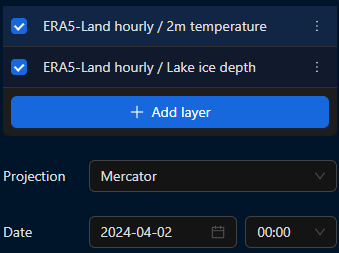
\includegraphics[width=0.3\textwidth]{assets/test4.png}
        	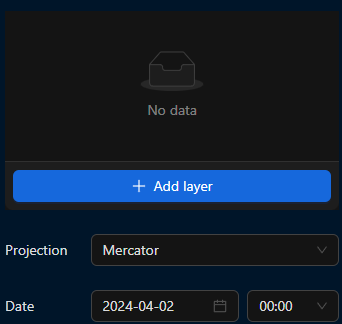
\includegraphics[width=0.3\textwidth]{assets/test5.png}
        	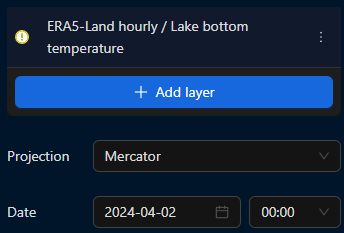
\includegraphics[width=0.3\textwidth]{assets/test6.png}
		}
		\caption{Снимки экрана}
	\end{figure}
	
	\subsection{Состав документации}
	Вся документация присутствует и соответствует стандартам.

\end{document}